\documentclass[12pt, class=article, crop=false]{standalone}
\usepackage[subpreambles=true]{standalone}
\usepackage[T1]{fontenc} % for font setting
\usepackage{tgtermes} % for font setting
\usepackage{import,
            graphicx,
            parskip,
            url,
            amsmath,
            wrapfig,
            soul}
\usepackage[most]{tcolorbox}
\usepackage[includeheadfoot,
            top=2.54cm,
            bottom=2.54cm,
            left=2.54cm,
            right=2.54cm]{geometry}%set margin
\usepackage[sort&compress]{natbib}
\setcitestyle{square}
\setcitestyle{comma}
\usepackage[font={sf, small}, labelfont={bf, small}]{caption}
\usepackage{fancyhdr}

\tcbuselibrary{breakable}
\bibliographystyle{bibstyle}

\begin{document}

\section*{Research Strategy}

\subsection*{Significance}

% Over the past century, biologists have been intrigued by how interacting organisms are assembled in a certain environment.
% This process, termed "community assembly," has crucial implications for human society's public health and sustainability.
% For example, the community structure of human gut microbes impacts the development of the host immune system and protection against pathogen invasion.
% Community assembly also plays a critical role in large-scale biological outcomes, such as the environmental restoration of degraded habitats in human-dominated landscapes.
% The effect of environmental restoration on ecological communities is contingent on how colonizing species reach the restored site, often defining the "success" of the restoration project that managers invest millions of dollars for implementation.
% Therefore, understanding the regulatory rules in community assembly (hereafter, "assembly rule") is fundamental to a broad range of biological phenomena.
% \ul{\emph{The proposed research will develop a novel statistical method that addresses unsolved methodological barriers}} to progressing community assembly research.

\textbf{Problem statement.}
% A central question in community assembly is whether the niche or neutral assembly rule dictates biological communities.
% The niche paradigm assumes that species differ in their biological traits such that abiotic environments determine the outcome of local species interactions.
% As such, this paradigm predicts that the interplay between species' traits and the environment leads to the convergence of community structure among similar habitats.
% On the contrary, the neutral paradigm assumes the biological equivalence among species within a given community.
% Under the neutral scenario, community dynamics are highly sensitive to stochastic factors (e.g., species' immigration history) because the outcome of species interactions is analogous to a flip of a fair two-sided coin; the probability of being the winner is equal among species.
% The resultant community structure is unpredictable and can diverge even among otherwise identical habitats. Discerning assembly rules has practical importance.
% For example, maintaining specific gut conditions may yield desired microbe communities \emph{only if} they are strongly structured via niche mechanisms. Hence, resolving the ``niche vs. neutral" debate represents a major contribution to basic and applied biological sciences.

% Decades of the niche vs. neutral debate led to a general agreement that the dichotomous argument is inappropriate; both mechanisms act in concert to form observed biological communities.
% This finding has motivated researchers to explore environmental drivers of their relative importance in natural systems, and several influential hypotheses have emerged.
% Nonetheless, we argue that the state of knowledge in community assembly remains equivocal because \ul{\emph{a fundamental methodological issue is unsolved}}.
% Current statistical methods exploit information from \emph{spatial} community data (i.e., community structure among spatially separated localities) to discern niche and neutral assembly mechanisms, and these approaches can be grouped into two broad categories: (i) the community-environment (CE) and (ii) the community randomization (CR) approaches.
% The CE approach builds on the idea that if niche mechanisms are dominant, environmental similarity should explain the similarity in community structure among localities; unexplained variation is considered a sign of neutral mechanisms. Yet, this approach has been criticized because it is unrealistic to fully represent the species' niche dimensions with available environmental data. Meanwhile, the CR approach is robust to this problem. In this approach, we interpret that observed communities are niche-structured if their structure deviates from what would be expected under species' random distributions (i.e., the null model). While this method seems to overcome the aforementioned critique elegantly, a careful examination unveiled that non-random species' distributions can emerge through either niche or neutral mechanisms; thus, it is unclear that any deviations from random species distributions truly mean ``niche structured." Consequently, no existing method can measure the contributions of niche and neutral assembly rules from unmanipulated observational data.

\textbf{Solution.}
% Our proposal is motivated by the fact that \ul{\emph{time series data may provide deeper insights}} into community assembly rules. In theory, assembly rules are defined by the variation in species' traits within a given community, which dictates characteristic patterns of temporal community dynamics. In particular, niche and neutral communities show distinct signs of frequency dependency in species' population growth. If niche-structured, species' niche differences underpin the predominance of negative frequency dependence (= rarer species have greater population growth) such that rarer species can sustain populations; thus, the same set of species is likely to persist as far as the defining environments of species interactions remain similar. The neutral assembly, in contrast, lacks negative frequency dependency, facilitating the probabilistic mono-dominance of any species. Therefore, it is natural to expect that we may find a clear sign of assembly rules in time series data.

% \ul{\emph{Here, we propose a new method that leverages this attribute of time series data}} to understand assembly rules. In Specific Aim 1, we will design a groundwork that derives a theoretical backbone of this novel method. In Specific Aim 2, we will assess the performance of the developed method using experimental yeast communities, in which we manipulate the strength of niche and neutral mechanisms. In Specific Aim 3, we combine the developed method with accumulating global time series of community data to ask: "\emph{What controls the relative importance of niche vs. neutral mechanisms in natural systems?}" In the long term, our contributions will help improve the public health and the sustainability of natural resources by illuminating the fundamental mechanisms of community assembly.

\subsection*{Innovation}
% Understanding assembly rules has far-reaching implications for human society's sustainability as it relates to human health, food production, and biodiversity conservation, to name just a few. We assert that our proposal will advance this research field significantly through three important breakthroughs. First, \ul{\emph{our proposal is conceptually innovative}} because our new method has the potential to find novel results that contrast previous findings. As mentioned, current statistical methods in community assembly contain fundamental limitations in distinguishing niche mechanisms from neutral ones with observational data. The new method solves this issue with the possibility of reaching conclusions overturning the fundamental wisdom of community assembly research. Second, \ul{\emph{our proposal is methodologically innovative}} because the proposed method is highly robust to the inherent complexity of community data. A major challenge in community assembly research is the curse of dimensionality -- as the number of species increases, the non-linear system dynamics become so complicated that traditional statistical approaches are unhelpful. The proposed method derives analytically that community-wide information can be condensed into a single parameter; this unique simplification allows us to use ordinary statistics to quantify the contributions of niche and neutral mechanisms. Lastly, \ul{\emph{our method is applicable, in principle, to a broad range of biological systems, from microscopic to gigantic organisms}}. This property allows for cross-taxonomic and cross-ecosystem comparisons of assembly rules. Hence, this proposal has three innovative qualities that meet the NIH review criterion "\emph{Does the application challenge and seek to shift current research or clinical practice paradigms by utilizing novel theoretical concepts?}"

\subsection*{Approach}

\subsubsection*{Specific Aim 1: Development of a new modeling approach}

\textbf{The overarching goal of this aim is to develop a new modeling approach that identifies communities sensitive to priority effects.}
To this end, we will perform the following activities:
[1a] Derive a theoretical backbone for a statistical method that identifies sensitive communities.
[1b] Validate the performance of the proposed method with simulation experiments.

\textbf{Activity 1a: Development of a new statistical method}

\textbf{\textit{Goal}} -- 
Our goal in this activity is to derive a theoretical backbone for a statistical method that identifies sensitive communities.
In competitive communities, their sensitivity to priority effects is largely determined by the balance between intraspecific and interspecific competition, which are defined as the per-capita impact on population growth over time.
Therefore, a critical first step is to obtain reliable estimates of competition parameters through an empirical time series.
However, in empirical settings, it is often infeasible to directly estimate those parameters because of the ``\textit{curse of dimensionality}:'' as the number of species $S$ in the community increases, the length of the time series required for estimation increases exponentially.
Here, we propose a robust statistical method that solves this issue -- \ul{our method can estimate the balance of intra- and interspecific competition, regardless of the number of species, by capitalizing the fact that species-level competition can be condensed into an aggregate effect of the total community density.}

\textbf{\textit{Method detail: theoretical backbone}} -- 
As a true state of community dynamics over time, we consider a discrete recursion equation. The population density of species $i$ at time $t$, $x_{t,i}$ is modeled as:

\begin{equation}
\label{eq:m0}
x_{t + 1, i} = x_{t, i} f(x_{t, i}).
\end{equation}

$f(\cdot)$ is the function defining the per-capita population growth rate.
Although the method we propose here applies to any functions that assume linear combinations of species interaction terms, let us use a Ricker model as an example (we drop the subscript $t$ from $x_{t,i}$ to simplify the expression):

\begin{equation}
\label{eq:ricker}
f(x_{i}) = \exp(r_{0,i} - \alpha_i x_i - \sum_{j \ne i} \beta_{ij} x_{j}),
\end{equation}

where $r_{0,i}$ is the intrinsic population growth, $\alpha_{i}$ the intraspecific competition coefficient, and $\beta_{ij}$ the interspecific coefficient.
Here, we assume that $\beta_{ij}$ is randomly drawn from a given probability distribution, resulting in a sample mean ($\mu_{\beta}$) and SD ($\sigma_{\beta}$). 
Denoting the total community density as $x_T$ ($x_T = \sum_i x_i$), Equation \ref{eq:m0} can be reorganized to:

\begin{equation}
\label{eq:rickermod}
f(x_i) = \exp\left[g_i - (\alpha_i - \mu_{\beta} - \sigma_{\beta} \phi_i) x_i - (\mu_{\beta} + \sigma_{\beta} \phi_i) x_T \right],
\end{equation}

where $g_i = r_{0,i} + \sigma_{\beta} \sum_{j \ne i} b_{ij} \sum_{k \ne i, j} x_{k}$ and $\phi_i = \sum_{j \ne i} b_{ij}$.
In Equation \ref{eq:rickermod}, the interspecific competition $\beta_{ij}$ is re-parameterized as $b_{ij} = (\beta_{ij} - \mu_{\beta}) \sigma_{\beta}^{-1}$. Since $b_{ij}$ is a random variable with a mean $0$ and SD $1$, the expected value of the summation $E(\phi_i)$ is $\pm \sqrt{S - 1}$, where $S$ is the number of species in the community.

The re-organized function (Equation \ref{eq:rickermod}) has two important implications.
First, \ul{the function can be expressed as a function of two variables (species $i$'s density $x_i$ and the total community density $x_T$), substantially reducing the parameter dimension of the model.}
The original function (Equation \ref{eq:ricker}) parameterized competition effects by species, resulting in $S$ parameters of competition.
In contrast, in the re-organized equation, the competition effects are condensed into the aggregate effects of species $i$'s density ($\alpha_i - \mu_{\beta} - \sigma_{\beta} \phi_i$) and the total community density ($\mu_{\beta} + \sigma_{\beta} \phi_i$).

Second, \ul{the re-parameterization enables statistical inference of interspecific competition with relatively short time series data}.
Let $\gamma_i$ and $\delta_i$ be the effects of $i$'s population density and the total community density, respectively ($\gamma_i = -(\alpha_i - \mu_{\beta} - \sigma_{\beta} \phi_i)$ and $\delta_i = -(\mu_{\beta} + \sigma_{\beta} \phi_i)$).
Then, the log-transformed per-capita growth rate $\ln r_i$ becomes the following linear model:

\begin{equation}
\label{eq:rickerlog}
    \ln f(x_i) = \ln r_i = g_i + \gamma_i x_i + \delta_i x_T
\end{equation}

Thus, this re-parameterization greatly reduces the number of competition parameters from $S$ to two, \ul{regardless of the number of species in the community}.
As such, this modeling approach will solve the ``curse of dimensionality'' hindering the empirical time series analysis of community data.

\textbf{\textit{Method detail: null model analysis}} --
The community's sensitivity to priority effects is strongly affected by the balance between intra- and interspecific competition.
In this context, Equation \ref{eq:rickerlog} offers a promising avenue to simplify community data analysis. 
An intuitive statistical method would be to compare the effects of $x_i$ ($\gamma_i$) and $x_T$ ($\delta_i$) on $i$'s population growth (see Equation \ref{eq:rickerlog}).
However, this comparison is inappropriate because we cannot statistically separate the effect of intra- and interspecific competition (see Equation \ref{eq:rickermod}).
Consequently, we need an alternative approach to measure the balance of competition strength.

Here, \ul{we propose to use a neutral community to measure the sensitivity to priority effects.} 
A neutral community is comprised of ecologically identical species (intraspecific competition = interspecific competition); therefore, if the observed effect of $\delta_i$ is stronger (i.e., more negative) than what would be expected from the simulated neutral dynamics, the community should be sensitive to priority effects. Our proposed method proceeds with the following procedures:

\begin{enumerate}
    \item Estimate $\delta_i$ by fitting a linear statistical model to the observed population growth (see Equation \ref{eq:rickerlog}). We refer to this observed estimate as $\delta_{obs}$. While $\delta_{obs}$ can be estimated by species, we will average across species to reduce the uncertainty of parameter estimate.
    
    \item Estimate $\delta_i$ using simulated dynamics of a neutral community.
    We refer to this simulated estimate as $\delta_{null}$.
    A major advantage of this neutral approach is its feasibility of estimating the model parameters to simulate neutral dynamics. 
    Under the neutral scenario, all species obey the same recursion equation, leading to the following dynamics of the total community density $x_T$:

    \begin{align}
        \label{}
        x_{T, t+1} &= x_{T, t} \exp(\bar{r}_0 - \bar{\alpha} x_{T, t})\\
        \ln r_T &= \ln {x_{T, t+1}} - \ln {x_{T, t}} = \bar{r}_0 - \bar{\alpha} x_{T, t}.
    \end{align}

    As such, the key parameters for neutral simulation -- the intrinsic growth ($\bar{r}_0$) and competition strength ($\bar{\alpha}$) at the community level -- can be readily estimated with ordinary regression using the observed data of $x_T$.
    The simulated data will have a time series length identical to the observed data. 
    
    \item Approximate the probability of $\delta_{obs} < \delta_{null}$ [hereafter, $\Pr(\delta_{obs} < \delta_{null})$]. To approximate the probability, we produce $100 - 500$ simulated dynamics of a neutral community and yield $100 - 500$ estimates of $\delta_{null}$. $\Pr(\delta_{obs} < \delta_{null})$ will be calculated as the proportion of simulation replicates satisfying $\delta_{obs} < \delta_{null}$.
\end{enumerate}

\textbf{Activity 1a: Simulation experiment}

\textbf{\textit{Goal}} -- 
The proposed method in Activity 1a provides a framework to identify communities sensitive to priority effects. The goal of this activity is to validate the performance of this method using simulation experiments.
\ul{We will use time series data simulated with known competition and other parameters so that we can validate the relationship between the true sensitivity to priority effects and the proposed statistic $\Pr(\delta_{obs} < \delta_{null})$}.

\textbf{\textit{Method detail: simulation experiment (preliminary analysis)}} -- 
To validate the performance of the proposed null model analysis, we performed a simulation experiment. In this simulation, we 

\begin{table}
    \centering
    \caption{Parameter values used in the preliminary sensitivity analysis.}
    \begin{tabular}{cll}
        Symbol & Interpretation & Value\\
        \hline
        $r_i$            & Intrinsic population growth  & 1.0 or $\mbox{Unif(0.9, 1.1)}$\\
        $\alpha_{i}$     & Intraspecific competition    & 0.01, 0.02\\
        $\beta_{ij}$     & Interspecific competition    & $\mbox{Normal}(\mu_{\beta}, \sigma_{\beta}^2)$\\
        $\mu_{\beta}$    & Average interspecific competition & $\alpha_i \times \{0, 0.25, ..., 1.50\}$\\
        $\sigma_{\beta}$ & SD interspecific competition & $\mu_{\beta} \times \{0,  0.25\}$\\
        \hline
    \end{tabular}
    \label{tab:my_label}
\end{table}

\textit{Method detail: simulation experiment (proposed analysis)} --

\begin{wrapfigure}{r}{0.6\textwidth}
    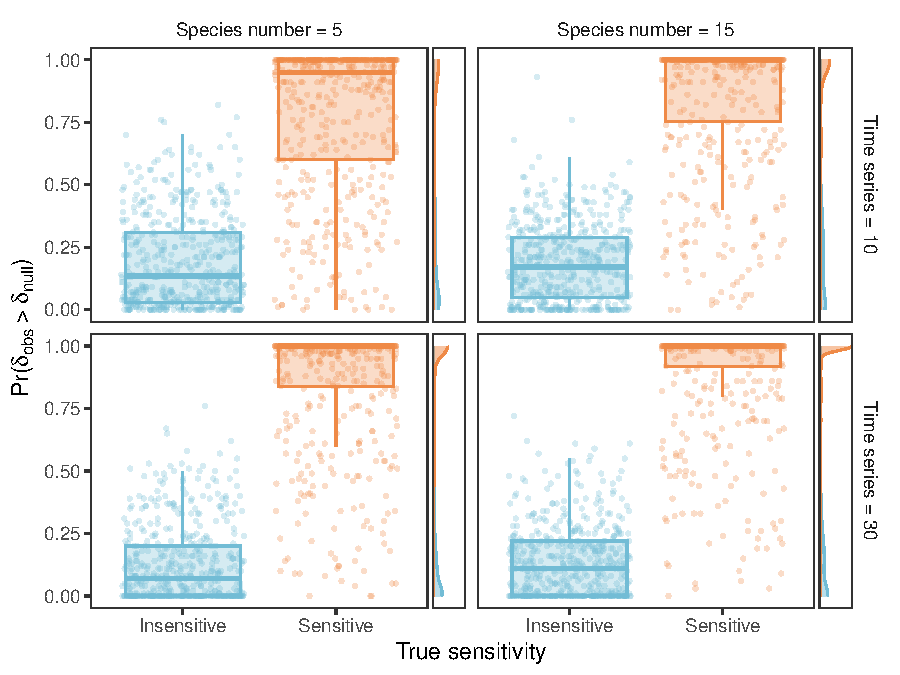
\includegraphics[scale=0.85]{output/figure_eigen.pdf}
    \caption{The proposed method captures the critical transition of community dynamics.}
    \label{fig:diffuse}
\end{wrapfigure}

text here 

% \begin{tcolorbox}[{
%   breakable,
%   colback=white,
%   colframe=gray,
%   coltext=black,
%   parbox=false,
%   boxsep=5pt,
%   arc=1pt}]

% \end{tcolorbox}

\end{document}
